\section{Sprint 6}
Im sechsten und letzten Sprint wurde diese beiden Stories bearbeitet:
\begin{itemize}
   \item Die Kommunikation mit den Stromzähler soll asynchron ausgeführt werden.
   \item SonarQube soll aufgesetzt werden und die gemeldete Code Smells bearbeitete werden.
\end{itemize}
Neben diesen Story wurde Zeit eingeplant, um bei den Nutzern der Anwendung ausführliches Feedback einzuholen.
Kleinere Änderungen und Bugfixes, welche aus dem Feedback hervorgehen sollen ebenfalls direkt im Sprint umgesetzt werden.
Die folgenden Abschnitte geben Auskunft über die erwähnten Arbeiten.

\subsection{Asynchrone Kommunikation}
\dq Die Kommunikation mit den Stromzähler soll asynchron ausgeführt werden.\dq
\subsubsection{Ziele}
Bisher funktioniert die Kommunikation mit den Zählern so, diese direkt im UI Thread ausgeführt wird.
Dies hat den Nachteil, dass die Benutzerschnittstelle während der Kommunikation eingefroren ist und nicht auf weitere Eingaben des Benutzers reagiert.
Ein weitere Nachteil der bisherigen Implementation ist, dass Kommunikationsfehler zu Abstürzen der ganzen Anwendung führen.
Das Ziel dieser Story ist es, die Kommunikation in einen Thread auszulagern und so asynchron auszuführen.
Dies soll Wert auf die Fehlertoleranz der Implementation gelegt werden.


\subsubsection{Vorgehen \& Schwierigkeiten}
In \ref{atsUmsetztung} wurde erklärt, wie der Code des \ac{ATS} eingebunden wurde.
Bisher war das Befehlsinterpreter Projekt eine direkte Abhängigkeit des DlmsQuickAccess.Dlms Projekts.
Die benötigten Klassen wurden dort instanziiert und verwendet. 
Dies führt dazu, dass DlmsQuickAccess.Dlms stark an den Befehlsinterpreter gekoppelt ist.
Ein Austausch des Kommunikationsstacks wäre mit grösseren Anpassungen verbunden.
Wie in Abschnitt \ref{portability} erklärt wurde, sind dies Anzeichen von tiefer Portabilität.

\begin{figure}[H]
   \centering
   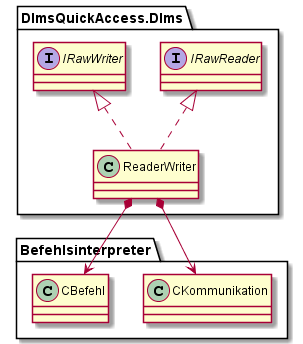
\includegraphics[width=0.5\textwidth]{gfx/dlms_vorher.png}
   \caption{
      Reduziertes Klassendiagramm um die ReaderWriter Klasse vor der Dependency Inversion
   }
   \label{fig:dlms_vorher}
\end{figure}

Da in diesem Sprint Änderungen am Kommunikationscode, also an DlmsQuickAccess.Dlms, geplant sind, wurde als erstes die zuvor genannte Kopplung bereinigt.
Dazu wurde das Dependency Inversion Principle angewendet.
Dieses besagt, dass High-Level-Module nicht von Low-Level-Modulen abhängen sollen.
Beide sollten von Abstraktionen abhängig sein \parencite{madasu35solid}.
Das Klassendiagramm in Abbildung \ref{fig:dlms_vorher} zeigt, wie die Klasse ReaderWriter von Klassen des Befehlsinterpreter abhängig ist.
Wie die Abhängigkeiten nach dem Refactoring nach Dependency Inversion Principle aussehen, ist in Abblidung \ref{fig:dlms_nachher} gezeigt.
Mit dem ICommunicator Interface definiert DlmsQuickAccess.Dlms nun lediglich die Schnittstelle eines Objekts, welches vom ReaderWriter benötigt wird.
Dieses wird mit der Communicator Klasse implementiert. Eine Instanz dieser Klasse kann nun in den ReaderWriter injected werden.
Somit wurde die Koppelung von DlmsQuickAccess.Dlms und Befehlsinterpreter aufgelöst.

% evtl schreiben, wo Communicator instantiert wird



\begin{figure}[H]
   \centering
   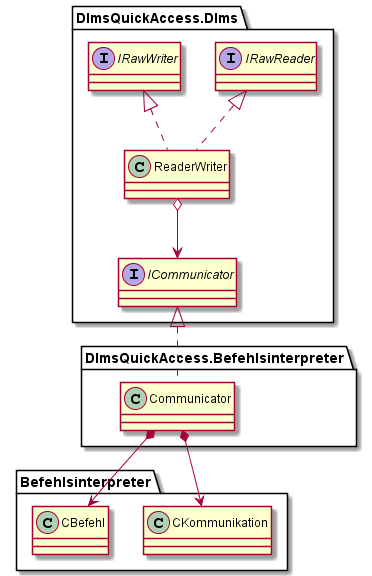
\includegraphics[width=0.5\textwidth]{gfx/dlms_nachher.png}
   \caption{
      Reduziertes Klassendiagramm um die ReaderWriter Klasse nach der Dependency Inversion
   }
   \label{fig:dlms_nachher}
\end{figure}

\subsubsection{states oder}

Kommunikation Asynchron machen
Bisher wird bei Kommunikation mit dem Zähler das UI eingefrohren
Wenn Kommunikation fehlschlägt stürtzt die Anwendung ab.
Kommt immer dan vor, wenn TLS Verbindung zuvor nicht sauber beendet wurde.

Die verschiedenen Zustände der Kommunikation soll mit dem State Pattern implementiert werden.
Das State Pattern ermöglicht, dass sich das Verhalten eines Objekts basierend auf dessen Zustand verändert \parencite{designPatterns}
Die Kommunikation kann mehrere Zustände haben:
\begin{itemize}
   \item Uninitiert
   \item Initiert
   \item Kommunizierend
   \item Fehlerzustand
\end{itemize}
Je nach Zustand muss sie anders auf neue Anfragen reagieren.
Ist sie beispielsweise noch uniniteiert, muss sie zuerst initiert werden, bevor die eigentliche Anfrage kommuniziert werden kann.
Vom kommunizierenden Zustand ist es möglich, dass sie in einen Fehlerzustand gerät.
Um diesen zu verlassen muss erneut initiert werden.
Abblidung TODO zeigt auf, wie diese Zustände mithilfe des State Patterns implementiert wurden.

\subsubsection{Schwierigkeiten}
% Bsp. ReadyState bekommt Read() befehl.
% -> Startet Read via ICommunicator des contexts.
% -> Sets Next state auf Communicating state

% IsCommuncating state erwartet die antwort des Reads.
% Beantwortet den das await des ursprünglichen callers.
% setzt zurück auf ReadyState
% -> kann jedoch auch ein stop erhalten während des warten
%    -> antwortet await ebenfalls (mit exception)
ATS Code nutz intern System.CurrentThread.Name für das Session Management.
Das Desing der Applikation sieht jedoch vor, dass die Kommunikation in Tasks ausgelagert wird.
Dann ist der Thread Name jeweils ein andere, als wenn aus dem UI oder Main Thread zugegriffen wird.

Lösung "1"



% \subsubsection{Bereinigung der internen Abhänigkeiten}
% "Sync Namespaces" sehr hilfreich.





\subsection{SonarQube}\label{s6:sonar}
Im Abschnitt \ref{quality:sonar} wurde das Tool SonarQube erklärt und festgehalten, dass es von der Landis+Gyr als bevorzugtes Software-Qualitatssicherungstool evaluiert wurde.
Zum Zeitpunkt dieser Arbeit verfügte die Landis+Gyr noch über keine laufende Instanz von SonarQube.
Deshalb wurde eine solche lokal auf dem Rechner des Entwicklers aufgesetzt.
Dies hat den Nachteil, dass ein Aufbau, wie er in Abschnitt \ref{sonar:funktionsweise} beschrieben ist nicht möglich ist.
Anstelle des \ac{CI} Servers muss der Build jeweils manuell ausgeführt und an die lokale SonarQube Instanz übermittelt werden.
Für dieses Projekt stellt dies kein Problem dar, da nur ein einzelner Entwickler am Code arbeitet.




% dotnet sonarscanner begin /k:"DlmsQuickAccess_NoATS" /d:sonar.host.url="http://localhost:9000"  /d:sonar.login="8568d95955df20f319cd05320e41bc4c8dac02f3"
% dotnet build DlmsQuickAccess_NoWinUI.sln
% dotnet sonarscanner end /d:sonar.login="8568d95955df20f319cd05320e41bc4c8dac02f3"

\subsection{Feedback}
Chakrit: 
- Landingscreen ist leer, wenn zuvor noch kein Produkt gestartet wurde. // auch von christoph
   - Wo finde ich einen Browser? // Chistoph
- Version nicht sichtbar im Loadingscreen
- Version nicht sichtbar im Log
- Wenn er via Windows startet steht im Log ein fehler.
- Enter to search

Someone:
- Lesen von Arrays stimmt nicht richtig
   - repro: Object list lesen

Christoph:
- Favoriten sind für mich eine Killerfeature
- Klartext der Enums auch ein Killerfeature

- Länge der Namen zu lang
- Cursor in Suchfeld nicht gut sichtbar
- Enter um Suche zu starten
- Feedback, dass kommunikation im Gange ist
- Feedback, wenn kommunikation fehlschlägt
- CHOICE type nicht supported
- Integers need to be correct length (leading 0)

DMT2 QuickAccess verwende ich nur noch, wenn bei einzelnen Attribtue/Objekte die im DlmsQuickAccess nicht richtig funktionieren.
   Wünsche mir, dass die Applikation weiterentwickelt wird und von der Firma den nötigen Support erhält.



Ronny:
- Bug, dass app crasht, wenn Description nicht vorhanden
- Beim Auslesen von Arrays mit vielen Einträgen wird das UI schnell unübersichtlich.
- Eines wäre praktisch, wenn genesene Werte als Datei gespeichert werden könnten. Z.B. Yaml.
- Starten der Anwendung sehr Praktisch. Suchen in Windows nach "DlmsQuickAccess", Click auf das gewünschte Produkt und schon ist alles einsatzbereit.
Beim DMT2 wusste man nie, welche Konfiguration gerade geladen war und das ändern dieser ist jeweils umständlich.
- Die Schreib und Lesegeschwindigkeit ist eindrücklich.
